% Source: AESP_466_ClassWork/Supplements/Notes/latex/5.1.3/5.1.3.tex

\documentclass[border=4pt]{standalone}
\usepackage{amsmath,amssymb,amsthm}
\usepackage{graphicx}
\usepackage{tikz}
\usepackage{xcolor}
\usetikzlibrary{arrows.meta,calc,positioning,decorations.markings,patterns,shapes.geometric,angles,quotes,3d}

\definecolor{Garnet}{HTML}{73000A}
\definecolor{USC_Rose}{HTML}{CC2E40}
\definecolor{USC_Blue}{HTML}{466A9F}
\definecolor{USC_Slate}{HTML}{1F414D}
\definecolor{USC_Olive}{HTML}{65780B}
\definecolor{USC_Lime}{HTML}{CED318}
\definecolor{USC_Gold}{HTML}{A49137}
\definecolor{USC_Black90}{HTML}{565556}
\definecolor{USC_Black10}{HTML}{ECECEC}

\newcommand{\vect}[1]{\mathbf{#1}}
\newcommand{\mat}[1]{\mathbf{#1}}
\newcommand{\uvec}[1]{\hat{\mathbf{#1}}}
\newcommand{\transpose}{^{\mkern-1.5mu\mathsf{T}}}
\newcommand{\inv}{^{-1}}
\newcommand{\deriv}[2]{\frac{d #1}{d #2}}
\newcommand{\pderiv}[2]{\frac{\partial #1}{\partial #2}}

\begin{document}
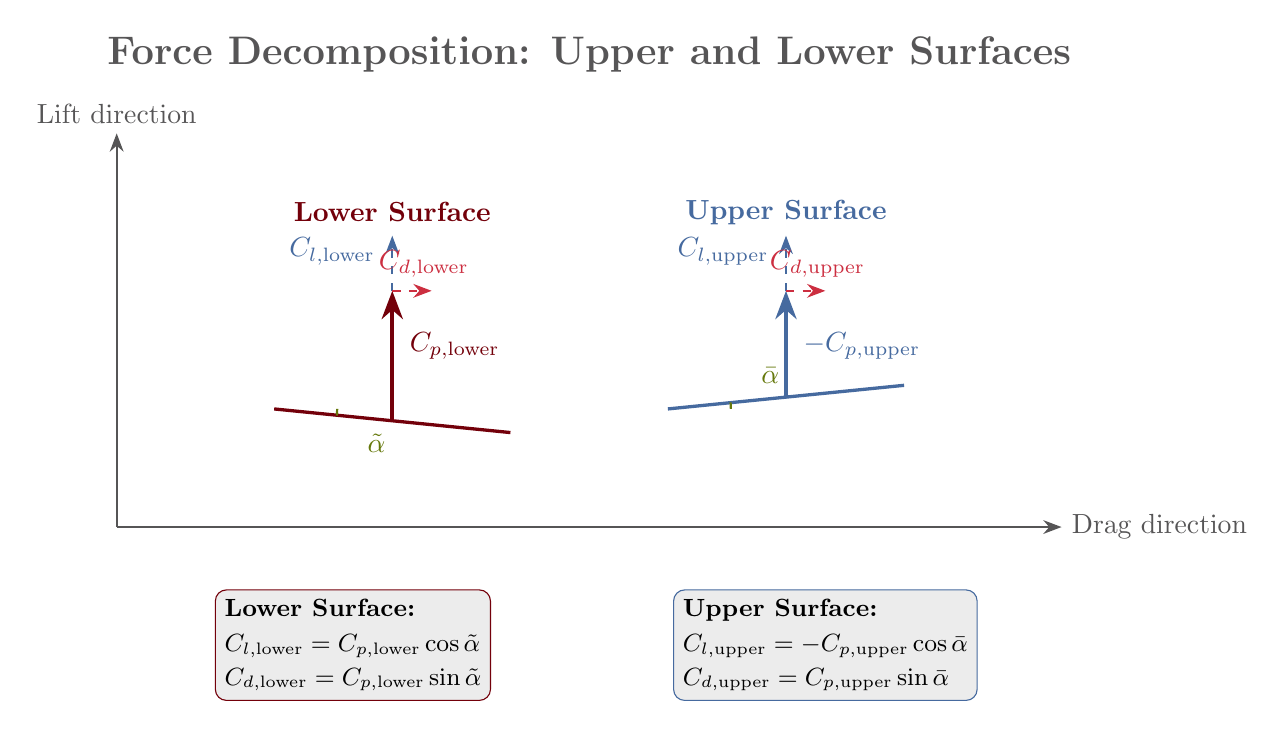
\begin{tikzpicture}[>=Stealth, scale=1.0]
    % Title
    \node[font=\Large\bfseries, USC_Black90] at (6,6) {Force Decomposition: Upper and Lower Surfaces};

    % Coordinate system
    \draw[->, thick, USC_Black90] (0,0) -- (12,0) node[right] {Drag direction};
    \draw[->, thick, USC_Black90] (0,0) -- (0,5) node[above] {Lift direction};

    % Lower surface panel
    \begin{scope}[shift={(2,1.5)}]
        \node[font=\bfseries, Garnet] at (1.5,2.5) {Lower Surface};

        % Surface line
        \draw[very thick, Garnet] (0,0) -- (3,-0.3);

        % Pressure force (normal to surface)
        \draw[->, ultra thick, Garnet] (1.5,-0.15) -- (1.5,1.5);
        \node[Garnet, right] at (1.6,0.8) {$C_{p,\text{lower}}$};

        % Angle annotation
        \draw[thick, USC_Olive] (0.8,0) arc[start angle=0, end angle=-6, radius=0.8];
        \node[USC_Olive, below] at (1.3,-0.2) {$\tilde{\alpha}$};

        % Component arrows
        \draw[->, thick, dashed, USC_Blue] (1.5,1.5) -- (1.5,2.2);
        \node[USC_Blue, left] at (1.4,2.0) {$C_{l,\text{lower}}$};
        \draw[->, thick, dashed, USC_Rose] (1.5,1.5) -- (2.0,1.5);
        \node[USC_Rose, above] at (1.9,1.55) {$C_{d,\text{lower}}$};
    \end{scope}

    % Upper surface panel
    \begin{scope}[shift={(7,1.5)}]
        \node[font=\bfseries, USC_Blue] at (1.5,2.5) {Upper Surface};

        % Surface line
        \draw[very thick, USC_Blue] (0,0) -- (3,0.3);

        % Pressure force (suction, pointing away from surface)
        \draw[->, ultra thick, USC_Blue] (1.5,0.15) -- (1.5,1.5);
        \node[USC_Blue, right] at (1.6,0.8) {$-C_{p,\text{upper}}$};

        % Angle annotation
        \draw[thick, USC_Olive] (0.8,0) arc[start angle=0, end angle=6, radius=0.8];
        \node[USC_Olive, above] at (1.3,0.2) {$\bar{\alpha}$};

        % Component arrows
        \draw[->, thick, dashed, USC_Blue] (1.5,1.5) -- (1.5,2.2);
        \node[USC_Blue, left] at (1.4,2.0) {$C_{l,\text{upper}}$};
        \draw[->, thick, dashed, USC_Rose] (1.5,1.5) -- (2.0,1.5);
        \node[USC_Rose, above] at (1.9,1.55) {$C_{d,\text{upper}}$};
    \end{scope}

    % Summary equations
    \node[draw=Garnet, fill=USC_Black10, rounded corners, align=left, font=\small] at (3,-1.5) {
        \textbf{Lower Surface:}\\[0.2em]
        $C_{l,\text{lower}} = C_{p,\text{lower}}\cos\tilde{\alpha}$\\[0.1em]
        $C_{d,\text{lower}} = C_{p,\text{lower}}\sin\tilde{\alpha}$
    };

    \node[draw=USC_Blue, fill=USC_Black10, rounded corners, align=left, font=\small] at (9,-1.5) {
        \textbf{Upper Surface:}\\[0.2em]
        $C_{l,\text{upper}} = -C_{p,\text{upper}}\cos\bar{\alpha}$\\[0.1em]
        $C_{d,\text{upper}} = C_{p,\text{upper}}\sin\bar{\alpha}$
    };

\end{tikzpicture}
\end{document}
